\documentclass[9pt,twocolumn,twoside]{osajnl}

\journal{jocn} 

% Set the article type for journal submissions. Comment out this line for Optica Open preprint submissions.
\setboolean{shortarticle}{false}
% true = letter / tutorial
% false = research / review article

\title{\LaTeX\  template for preparing a research article for submission to the \emph{Journal of Optical Communications and Networking}}

\author[1,2,3]{Author One}
\author[2,*]{Author Two}
\author[1]{Author Three}

\affil[1]{Publications Department, Optica Publishing Group, 2010 Massachusetts Avenue NW, Washington DC, 20036, USA}
\affil[2]{School of Science, University of Technology, 2000 J St. NW, Washington DC, 20036, USA}
\affil[3]{School of Optics, University of Technology, 2000 J St. NW, Washington DC, 20036, USA}

\affil[*]{email@my-email.com}

%% To be edited by editor
% \dates{Compiled \today}

%% To be edited by editor
% \doi{\url{http://dx.doi.org/10.1364/XX.XX.XXXXXX}}

\begin{abstract}
JOCN article style and format is being updated to conform to Optica journal style and format. This new template is now required for preparing a research article for submission to the \emph{Journal of Optical Communications and Networking}. Consult the \href{https://www.opg.optica.org/submit/templates/}{Author Style Guide} for general information about manuscript preparation. Authors may also \href{https://opticaopen.org}{submit articles} prepared using this template to the Optica Publishing Group preprint server, \href{https://preprints.opticaopen.org}{Optica Open}. However, doing so is optional. Please refer to the submission guidelines found there. Note that copyright and licensing information should no longer be added to your Journal or Optica Open manuscript.
\end{abstract}

\setboolean{displaycopyright}{false} % Do not include copyright or licensing information in submission.

\begin{document}

\maketitle

\section{Introduction}
This  template is designed to assist with creating an article to submit to the \emph{Journal of Optical Communications and Networking}. See the \href{https://opg.optica.org/submit/templates/}{Style Guide} and \href{https://www.opg.optica.org/submit/templates/}{Manuscript Templates} pages for more details.

If you have a question while using this template on {Overleaf}, please use the help menu (``?'') on the top bar to search for help or ask us a question using our \href{https://www.overleaf.com/contact}{contact form}.

\section{Corresponding author}

We require manuscripts to identify a single corresponding author. The corresponding author typically is the person who submits the manuscript and handles correspondence throughout the peer review and publication process. If other statements about author contribution and contact are needed, they can be added in addition to the corresponding author designation.

%Example with the corresponding author designated by an asterisk:

%\author{Author One\authormark{1} and Author Two\authormark{2,*}}

%\address{\authormark{1}Peer Review, Publications Department,
%Optica Publishing Group, 2010 Massachusetts Avenue NW,
%Washington, DC 20036, USA\\
%\authormark{2}Publications Department, Optica Publishing Group,
%2010 Massachusetts Avenue NW, Washington, DC 20036, USA\\
%%\authormark{3}xyz@optica.org}

%\email{\authormark{*}opex@optica.org}}

% Example with the corresponding author designated by an asterisk and a note indicating equal contributions by two authors.

%\author{Author One\authormark{1,3} and Author %Two\authormark{2,3,*}}

% \address{\authormark{1}Peer Review, Publications Department,
% Optica Publishing Group, 2010 Massachusetts Avenue NW, %Washington, DC 20036, USA\\
% \authormark{2}Publications Department, Optica Publishing Group, %2010 Massachusetts Avenue NW, Washington, DC 20036, USA\\
% \authormark{3}The authors contributed equally to this work.\\
%\authormark{*}opex@optica.org}}

% \section{Examples of Article Components}
% \label{sec:examples}

\section{Examples of Article Components}
\label{sec:examples}

The sections below show examples of different article components.

\section{Figures and Tables}

It is not necessary to place figures and tables at the back of the manuscript. Figures and tables should be sized as they are to appear in the final article. Do not include a separate list of figure captions and table titles.

Figures and Tables should be labelled and referenced in the standard way using the \verb|\label{}| and \verb|\ref{}| commands.

\subsection{Sample Figure}

Figure \ref{fig:falsecolor} shows an example figure.

\begin{figure}[htbp]
\centering
\fbox{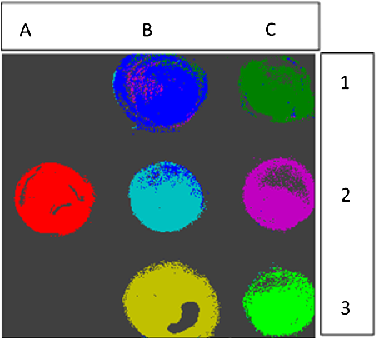
\includegraphics[width=.8\linewidth]{sample}}
\caption{False-color image, where each pixel is assigned to one of seven reference spectra.}
\label{fig:falsecolor}
\end{figure}

\subsection{Author Photographs}
Author photographs. The final printed size of an author photograph is exactly 1 inch wide by 1 1/4 inches long (6 picas × 7 1/2 picas). Please ensure that the author photographs you submit are proportioned similarly.

\subsection{Sample Table}

Table \ref{tab:shapefunctions} shows an example table.

\begin{table}[htbp]
\centering
\caption{\bf Shape Functions for Quadratic Line Elements}
\begin{tabular}{ccc}
\hline
local node & $\{N\}_m$ & $\{\Phi_i\}_m$ $(i=x,y,z)$ \\
\hline
$m = 1$ & $L_1(2L_1-1)$ & $\Phi_{i1}$ \\
$m = 2$ & $L_2(2L_2-1)$ & $\Phi_{i2}$ \\
$m = 3$ & $L_3=4L_1L_2$ & $\Phi_{i3}$ \\
\hline
\end{tabular}
  \label{tab:shapefunctions}
\end{table}

\section{Sample Equation}

Let $X_1, X_2, \ldots, X_n$ be a sequence of independent and identically distributed random variables with $\text{E}[X_i] = \mu$ and $\text{Var}[X_i] = \sigma^2 < \infty$, and let
\begin{equation}
S_n = \frac{X_1 + X_2 + \cdots + X_n}{n}
      = \frac{1}{n}\sum_{i}^{n} X_i
\label{eq:refname1}
\end{equation}
denote their mean. Then as $n$ approaches infinity, the random variables $\sqrt{n}(S_n - \mu)$ converge in distribution to a normal $\mathcal{N}(0, \sigma^2)$.

\section{Sample Algorithm}

Algorithms can be included using the commands as shown in algorithm \ref{alg:euclid}.

\begin{algorithm}
\caption{Euclid’s algorithm}\label{alg:euclid}
\begin{algorithmic}[1]
\Procedure{Euclid}{$a,b$}\Comment{The g.c.d. of a and b}
\State $r\gets a\bmod b$
\While{$r\not=0$}\Comment{We have the answer if r is 0}
\State $a\gets b$
\State $b\gets r$
\State $r\gets a\bmod b$
\EndWhile\label{euclidendwhile}
\State \textbf{return} $b$\Comment{The gcd is b}
\EndProcedure
\end{algorithmic}
\end{algorithm}

\section{Supplemental Material}

Consult the Author Guidelines for Supplementary Materials in Optica's Journals for details on accepted types of materials and instructions on how to cite them. For preprints submitted to Optica Open a link to supplemental material should be included in the submission, but do not upload the material.
All materials must be associated with a figure, table, or equation or be referenced in the results section of the manuscript.
(1) 2D and 3D image files and video must be labeled “Visualization,” not “Movie,” “Video,” “Figure,” etc.
(2) Machine-readable data (for example, csv files) must be labeled  “Data File.”  Number data files and visualizations consecutively, e.g., “Visualization 1, Visualization 2….”
(3) Large datasets or code files must be placed in an open, archival database.  Such items should be mentioned in the text as either “Dataset” or “Code,” as appropriate, and also be cited in the references list.  For example, “see Dataset 1 (Ref. [1]) and Code 1 (Ref [2]).” Here are examples of the references:

\subsection{Sample Dataset Citation}

1. M. Partridge, "Spectra evolution during coating," figshare (2014) [retrieved 13 May 2015], http://dx.doi.org/10.6084/m9.figshare.1004612.

\subsection{Sample Code Citation}

2. C. Rivers, "Epipy: Python tools for epidemiology," (figshare, 2014) [retrieved 13 May 2015], http://dx.doi.org/10.6084/m9.figshare.1005064.

\section{Funding and Acknowledgments}

Formal funding sources should be listed in a separate paragraph block before any other acknowledgment information. Funding sources and any associated grant numbers should match the information entered into the Prism manuscript system. Funders should be listed without any introductory language or use of labels (do not use labels such as “grant no.”). The acknowledgments may contain any information that is not related to funding. Here is an example:

\section*{Funding}National Science Foundation (NSF) (1263236, 0968895, 1102301); The 863 Program (2013AA014402).


\section*{Acknowledgments}The authors thank H. Haase, C. Wiede, and J. Gabler for technical support.

\section{References}

Full references (to aid the editor and reviewers) must be included. This will be produced automatically if you are using a .bib file.

\bigskip
\noindent Add citations manually or use BibTeX. See \cite{Chitimalla:17,Wen:16}.

% Bibliography
\bibliography{sample}


  
\end{document}
